\title{\vspace{160px} \textbf{\huge{Multimedia}} \\\vspace{17.5px} \LARGE{Homework 1}  \vspace{10px}}
\author{\href{https://github.com/imAlessas}{Alessandro Trigolo}}
\date{30 Aprile 2024}

\begin{document}

\maketitle\newpage

\tableofcontents
\listoffigures
\vspace{20px}
\newpage

\listoftodos\newpage


\section{Obiettivo}
\todo{Descrivi decentemente l'obiettivo}



\vspace{30px}\section{Codice sorgente}
\todo{Rifai introduzione}
Il linguaggio scelto per completare le richieste dell'homework è \texttt{Python}; all'interno del documento saranno presenti solo i punti salienti dello script, che comunque può essere ispezionato al seguente \href{https://github.com/imAlessas/computer-networks/blob/main/multimedia/hw-1/script/lossless_coding.py}{\texttt{link}}.



\vspace{15px}\subsection{Entropia dell'immagine}
La prima richiesta dell'homework è divisa in due macro parti, la prima richiede di selezionare e mostrare un'immagine mentre la seconda richiesta chiede di calcolare l'entropia dell'immagine.

L'immagine scelta è un'immagine di \textsl{Spider-Man} a colori, di conseguenza è necessario estrarne la luminaza per fara diventare in binaco e nero. Dopo aver caricato l'immagine a colori con l'opportuna funzione \texttt{imread} del pacchetto \texttt{matplotlib.image} è necessario usare la funzione \texttt{cvtColor} del pacchetto \texttt{cv2} di \texttt{opencv}. Il seguente script, dopo aver eseguito le suddette operazioni si occupa di mostrare le due immagini a schermo attraverso una \texttt{subplot}.

\begin{lstlisting}
# Prepare to load the image
img_file_name = "spiderman"
img_extension = ".jpg"
current_dir = os.getcwd()

# path to reach the img
path_to_img = os.path.join(current_dir, "multimedia", "hw-1", "script", "imgs") + "/"

# loads the colored image
img = mpimg.imread(path_to_img +  img_file_name + img_extension) 

# extracts the luminance
gray_img = cv2.cvtColor(img, cv2.COLOR_BGR2GRAY)

# creates a figure with two subplots
fig, axs = plt.subplots(1, 2, figsize=(12, 6))

# displays the colored image in the first subplot
axs[0].imshow(img, cmap='gray')
axs[0].set_title('Colored image')
axs[0].axis('off')

# displays the grayscale image in the second subplot
axs[1].imshow(gray_img, cmap='gray')
axs[1].set_title('Grayscale image')
axs[1].axis('off')
\end{lstlisting}

\noindent Dopo aver eseguito lo script soprastante si può notare che la luminanza dell'immgine è stata estratta con successo (figura \ref{fig:colored-grayscale}).

\begin{figure}[h]
    \centering
    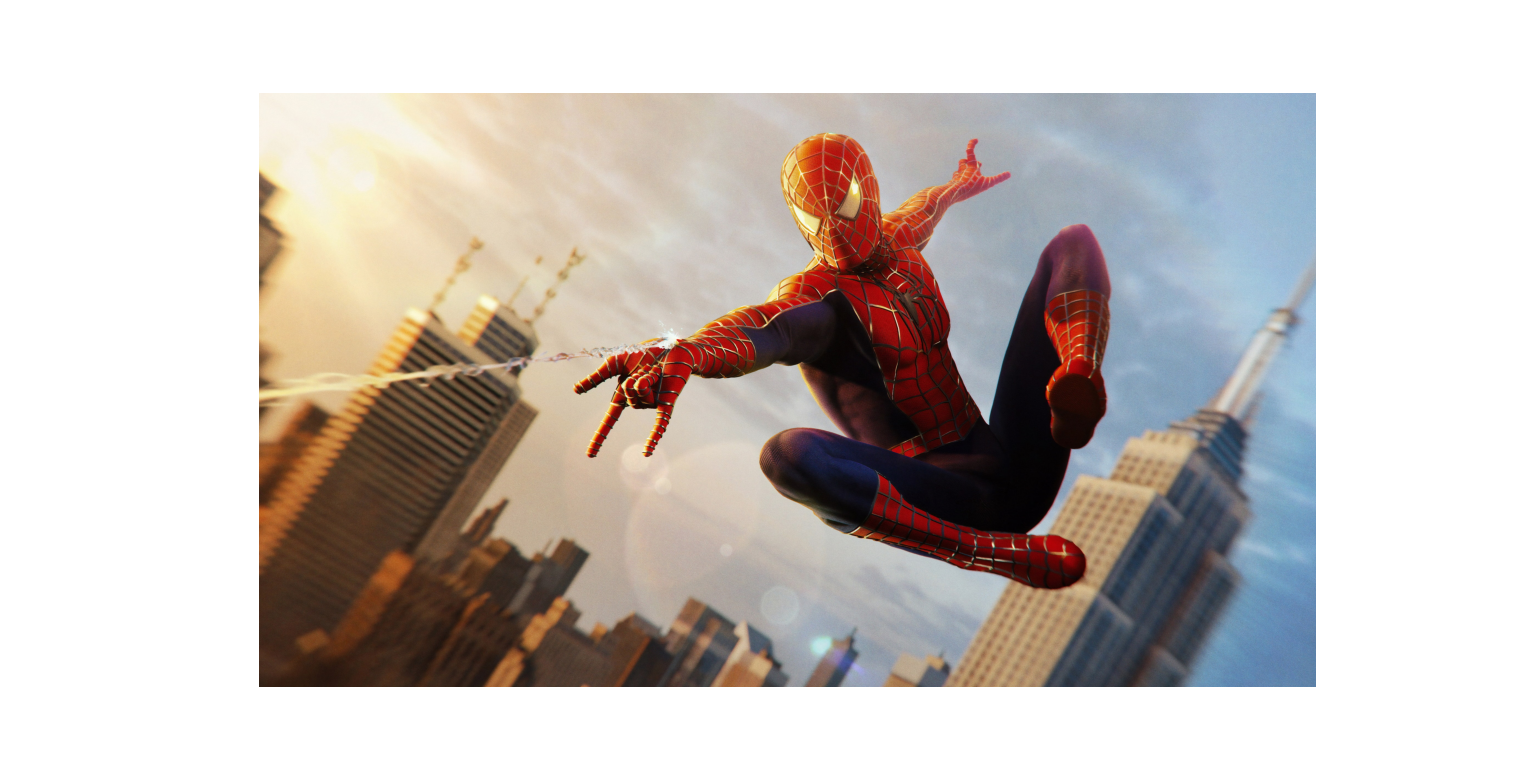
\includegraphics[width = .7\textwidth]{hw-1/report/imgs/colored.png}
    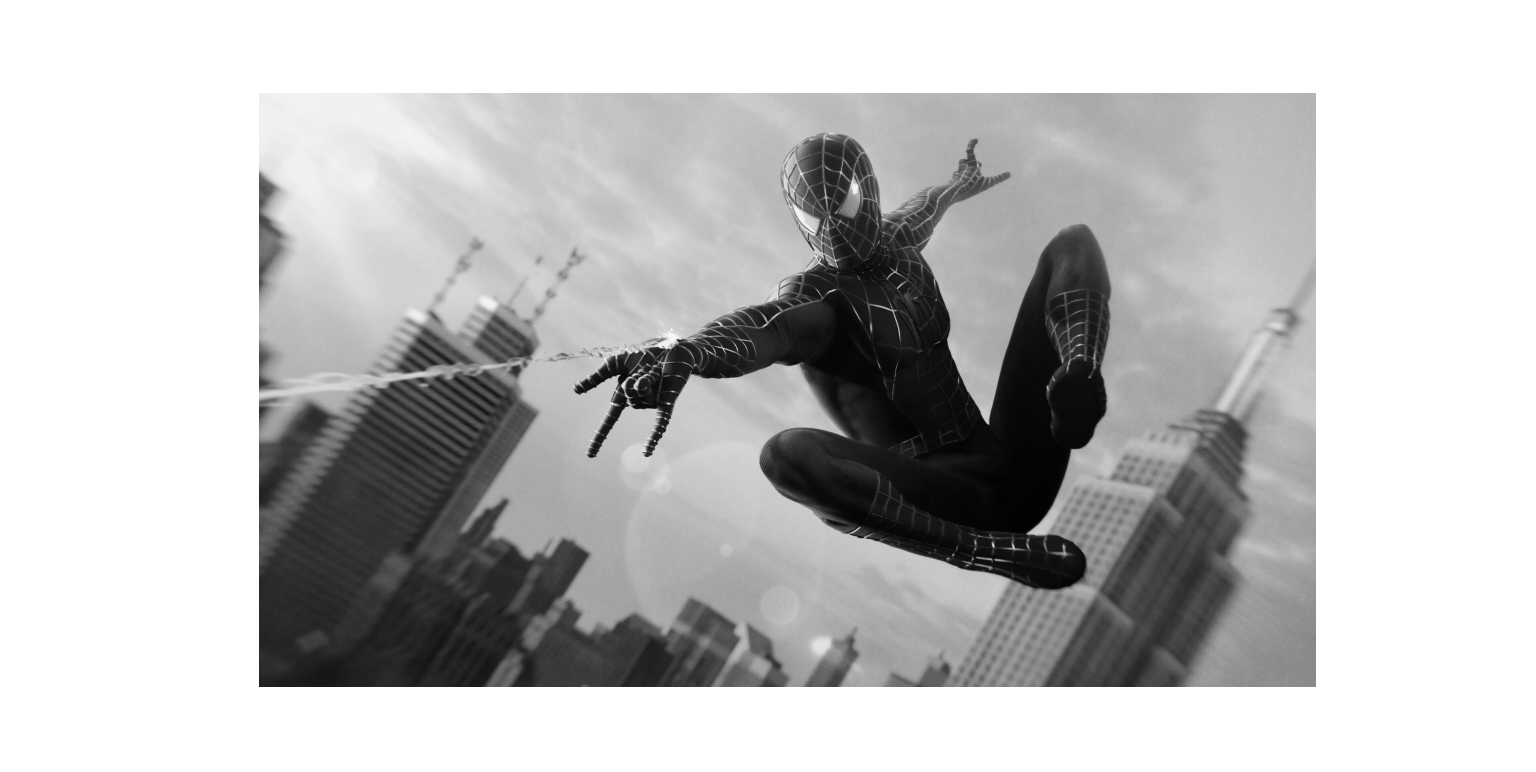
\includegraphics[width = .7\textwidth]{hw-1/report/imgs/grayscale.png}
    \caption{Estrazione della luminaza da una immagine a colori.}
    \label{fig:colored-grayscale}
\end{figure}

\FloatBarrier\noindent In secondo luogo è necessario calcolare l'entropia dell'immagine in bianco e nero. L'entropia di una variabile aleatoria $X$ (in questo caso l'immagine) è definita come l'\textbf{informazione media} degli eventi della sorgente; l'informazione di un evento è descritta dalla funzione seguente:

\begin{gather*}
    I(X) = \log_2\left( \frac{1}{p_i} \right)
\end{gather*}

\noindent Che è una variabile che diminuisce all'aumentare della probabilità dellevento $p_i$. Questo è ragionevole in quanto più un evento è imporbabile (quindi $p_i \to 0$) e più la sua informazione è alta ($I(X) \to +\infty$). Assumendo che gli eventi della sorgente siano indipendenti, l'informazione media si traduce nella seguente formula:

\begin{gather*}
    H(X) = E[I(X)] \, = \, \sum_{i = 1}^M p_i\log_2\left( \frac{1}{p_i} \right) \, = \, - \sum_{i = 1}^M p_i\log_2{p_i}
\end{gather*}

\noindent Dove con $M$ si indica il numero di elementi nell'insieme $X$. Questa formula si riassume nel seguente script, dove la variabile contenente l'immagine in bianco e nero viene trasposta e convertita in un vettore di pixel monodimensionale. In secondo luogo attraverso la funzione \texttt{numpy.histogram} vengono contate il numero di occorrenze per ogni valore di pixel. Successivamente, per calcolare la probabilità, si divide il numero di occorrezze per il numero totale di occorrenze, escludendo eventuali valori diversi da zero. Una volta calcolare la probabilità, attraverso le funzioni  \texttt{numpy.sum} e \texttt{numpy.log2} si ottiene il valore dell'entropia $H(X)$.


\begin{lstlisting}
# flatten the transposed matrix to read pixels row by row
raster_scan = np.transpose(gray_img).flatten()

# count the occurrences of each pixel value
occurrencies = np.histogram(raster_scan, bins=range(256))[0]

# calculate the relative frequencies
rel_freq = occurrencies / np.sum(occurrencies)

# remove zero-values of probability
p = rel_freq[rel_freq > 0]

# compute and display the entropy
HX = - np.sum(p * np.log2(p))
print(f"\nThe entropy of {img_file_name}{img_extension} is {HX:.3f} bpp")
\end{lstlisting}

\noindent Dopo aver eseguito lo script, l'entropia dell'immagine scelta è di \textbf{7.530 bpp}.





\vspace{15px}\subsection{Codifica con dizionario}
La seconda task chiede di utilizzare una compressione a dizionario, come \texttt{zip} nel caso di \textsl{Windows} per poi calcolare il \textsl{bitrate} risultante. Lo script necessario per soddisfare la richiesta è presentato nel frammento di codice sottostante. In particolare le prime due righe si occupano di "zippare" il file mentre le istruzioni seguenti estraggono la dimensione dell'immagine compressa (in bytes). Infine nelle ultime linee del frammento di codice viene computato l'effettivo \textsl{bitrate} dividendo la dimensione del file compresso con la dimensione dell'immagine originale, ottenuta tramite i valori di ritorno dell'attributo \texttt{img.shape}.

\begin{lstlisting}
# zip the image
cmd = f"zip {path_to_img}{img_file_name}.zip {path_to_img}{img_file_name}.jpg"
os.system(cmd)

# get the zip bytes
img_stats = os.stat(f"{path_to_img}{img_file_name}.jpg")
zip_bytes = img_stats.st_size

# get img size
height, width = gray_img.shape
img_size = width * height

# get the birate
zip_bitrate = zip_bytes * 8 / img_size 
print(f"\nThe bitrate of {img_file_name}.zip is {zip_bitrate:.3f} bpp\n")
    \end{lstlisting}

\noindent Dunque, dopo aver eseguito lo script si ottiene il valore del bitrate, corrispondente a \textbf{1.340 bpp}. 



\vspace{15px}\subsection{Discussione risultati parziali}\todo{migliora risposta task 3}
Il risultato trovato calcolando il bitrate della codifica con dizionario (1.340 bpp) è molto più basso rispetto al volore dell'entropia $H(X)$, calcolato nel primo punto (7.530 bpp), suggerendo che quindi la codifica con dizionario risulta efficace nel ridurre la quantità di informazione necessaria per rappresentare i dati, sfruttando le ridondanze presenti nel segnale.




\vspace{15px}\subsection{Codifica semplice}\label{simple-coding}
La quarta richiesta dell'homework è quella di effettuare una codifica predittiva \textsl{semplice}. In particolare, data l'immagine (che chiameremo $x(n)$), la codifica predittiva $y(n)$ è definita come segue:

\begin{gather*}
    y(n) = 
    \begin{cases}
        x(n) - 128 \hspace{37px} \text{se } \, n = 0 \\
        x(n) - x(n - 1) \hspace{15px} \text{altrimenti}\\
    \end{cases}
\end{gather*}

\noindent La suddetta codifica predittiva si traduce nel seguente Python script il quale, dopo aver calcolato la predizione, mostra l'immagine codificata.

\begin{lstlisting}
simple_coding_error = raster_scan[0] - 128
simple_coding_error = np.append(simple_coding_error, np.diff(raster_scan))

# plot error graph
plt.figure()
plt.imshow(np.transpose(np.reshape(np.abs(simple_coding_error), (width, height))), cmap = 'seismic')
plt.axis('image')
plt.axis('off')
plt.colorbar()
plt.title('Simple coding prediction error')
\end{lstlisting}

\noindent Dopo aver eseguito lo script soprastante si ottiene l'immagine mostrata nella figura \ref{fig:simple-coding}. Dall'immagine si può notare che le zone più rosse, ovvero le zone in cui il predittore ha fatto più errori, sono le zone dei contorni, come la skyline della città oppure lo stacco tra il personaggio raffigurato e il cielo. Questo perchè la differenza dei colori tra una sezione e l'altra è particolarmente accentuata. D'altro canto, le zone colorate di blu sono le zone dove i colori sono più uniformi: ecco quindi che i palazzi e il cielo sono per lo più dello stesso colore, suggerendo una zona dove la variazione di colore - e quindi di informazione - è molto bassa.

\begin{figure}[h]
    \centering
    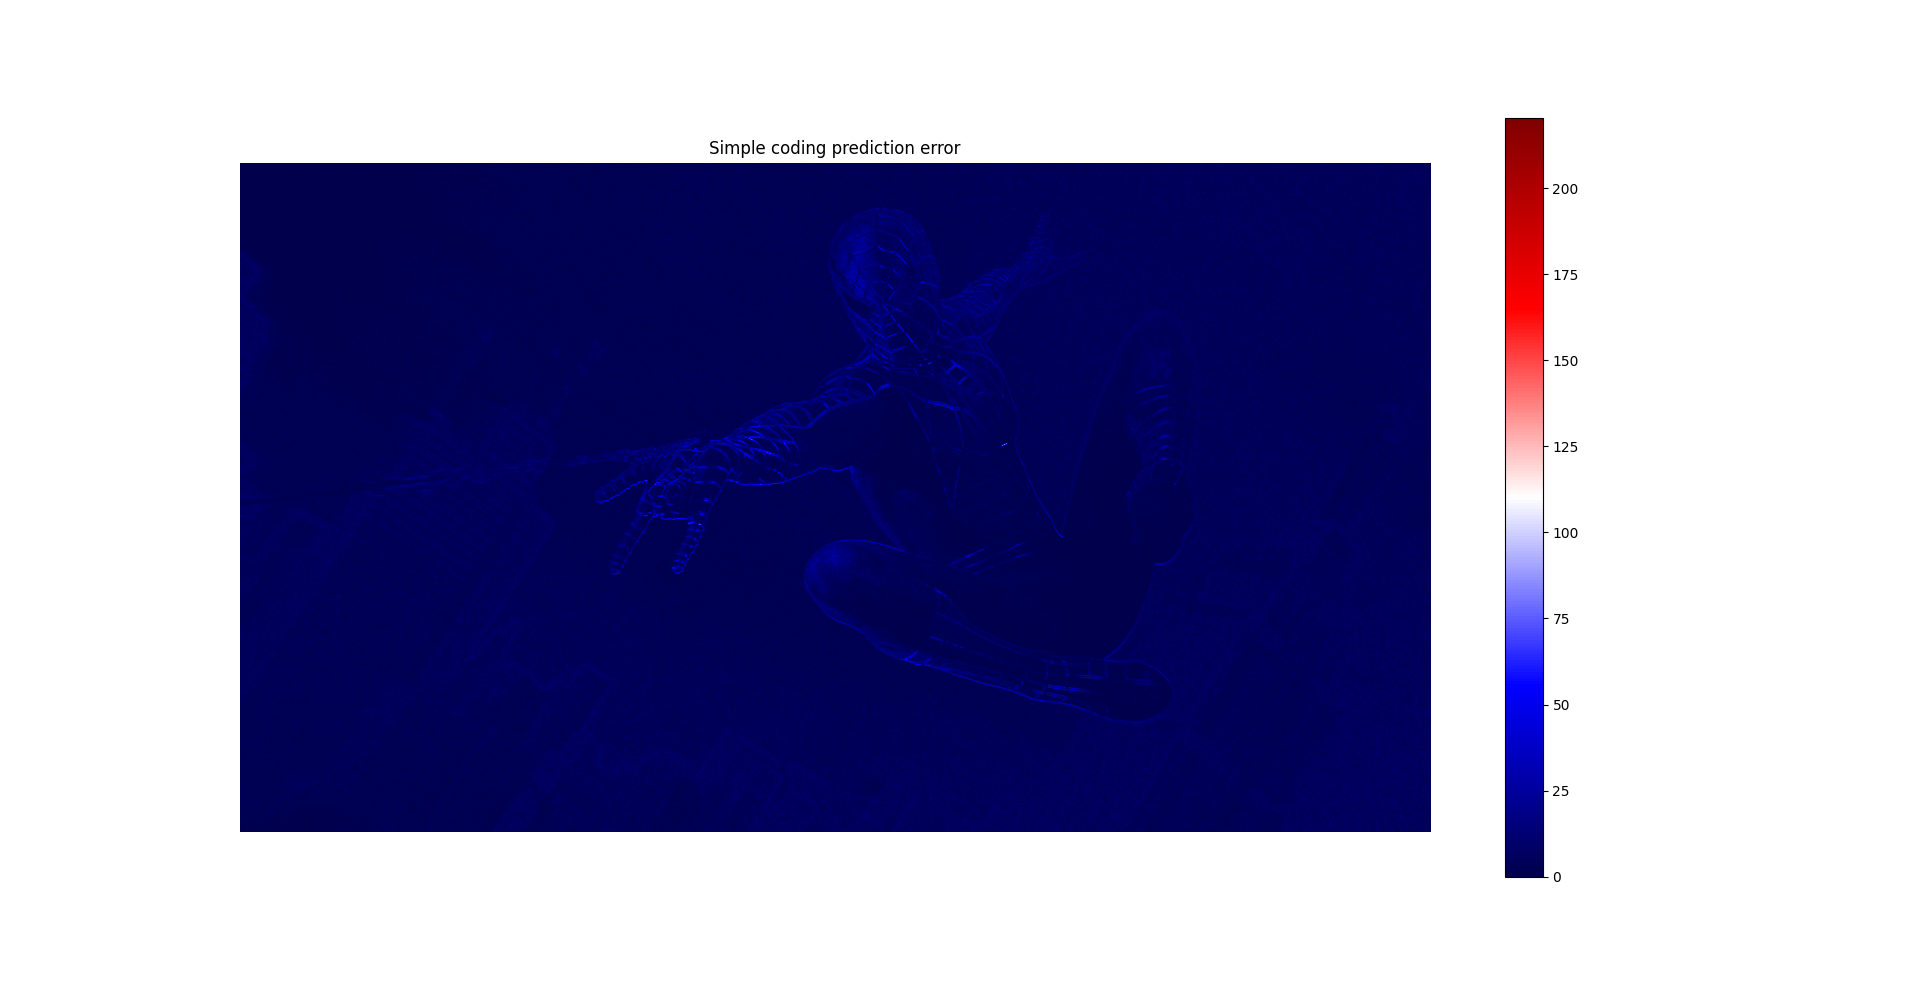
\includegraphics[width = .9\textwidth]{hw-1/report/imgs/simple-coding.png}
    \caption{Rappresentazione del modulo dell'errore di predizione nella codifica semplice.}
    \label{fig:simple-coding}
\end{figure}







\subsubsection{Analisi} \todo{valuta se farla subsection}
Seguedo le direttive della task numero 5 dell'homework, calcoliamo 

\todo{capisci cosa significa il valore EG-bpp}
\begin{lstlisting}
bit_count = 0
for symbol in simple_coding_error:
    codeword = exp_golomb_signed(symbol)
    bit_count += len(codeword)

exp_golomb_bpp = bit_count / img_size
print(f"The S-EG coding rate on prediction error is {exp_golomb_bpp:.4f}\n")    
\end{lstlisting}



\vspace{15px}\subsection{Codifica avanzata}

La penultima richiesta, esige di creare un nuovo tipo di codifica, detta \textsl{avanzata} definita come segue:

\begin{gather*}
    y(n, m) = 
    \begin{cases}
        x(n, m) - 128 \hspace{161px} \text{se } \, n = m = 0 \\
        x(n, m - 1) \hspace{171px} \text{se } \, n = 0\\
        x(n - 1, m) \hspace{171px} \text{se } \, m = 0\\
        \text{med}\left[ x(n, m - 1),\, x(n - 1, m),\, x(n - 1, m - 1) \right] \hspace{15px} \text{se } \, m = \text{MAX}\\
        \text{med}\left[ x(n, m - 1),\, x(n - 1, m),\, x(n - 1, m + 1) \right] \hspace{15px} \text{altrimenti}
    \end{cases}
\end{gather*} 

\noindent Dove in questo caso l'immagine anziche essere vista come un vettore $x$ è vista come una matrice di dimensione $n \times m$. Le richieste della codifica sono tradotte in uno script contenente due cicli annidati - il primo che itera lungo le righe della matrice e il secondo che itera lungo le colonne - dove allintero sono presenti una serie di \texttt{if} statement che soddisfano la definizione di codifica avanzata precedentemente citata. Inoltre si osserva la mediana dei tre valori è calcolata tramite una funzione definita dall'utente, descritta anch'essa all'interno dello script. 

\begin{lstlisting}
# median function for advanced coding
def median(a, b, c):
    vector = [a, b, c]
    vector.remove(min(vector))
    vector.remove(max(vector))
    
    return vector[0]



# blank image 
predicted_img = np.zeros_like(gray_img)

# iterates through the rows (height)
for row in range(height):

    # iterates through the cols (width)
    for col in range(width - 1):

        if row == 0 and col == 0:   # first pixel
            predicted_img[row][col] = gray_img[row][col] - 128
        
        elif row == 1:              # first row
            predicted_img[row][col] = gray_img[row][col - 1]
        
        elif col == 1:              # first col
            predicted_img[row][col] = gray_img[row - 1][col]
        
        elif col == (width - 1):    # last col
            predicted_img[row][col] = median(gray_img[row - 1][col], gray_img[row][col - 1], gray_img[row - 1][col - 1])

        else:                       # other cases
            predicted_img[row][col] = median(gray_img[row - 1][col], gray_img[row][col - 1], gray_img[row - 1][col + 1])

adv_coding_error = gray_img - predicted_img
\end{lstlisting}

\noindent Dopo aver eseguito lo script è possibile mostrare l'errore di predizione sottraendo l'immagine predetta \texttt{predicted\_img} con l'immagine iniziale \texttt{img} e "plottando" il suo valore assoluto come segue mediante uno script simile a quello mostrato per la codifica semplice (\ref{simple-coding}). L'immagine mostrata in figura \ref{fig:advanced-coding} è ciò che risulta degli errori commessi durante la predizione.

\begin{figure}[h]
    \centering
    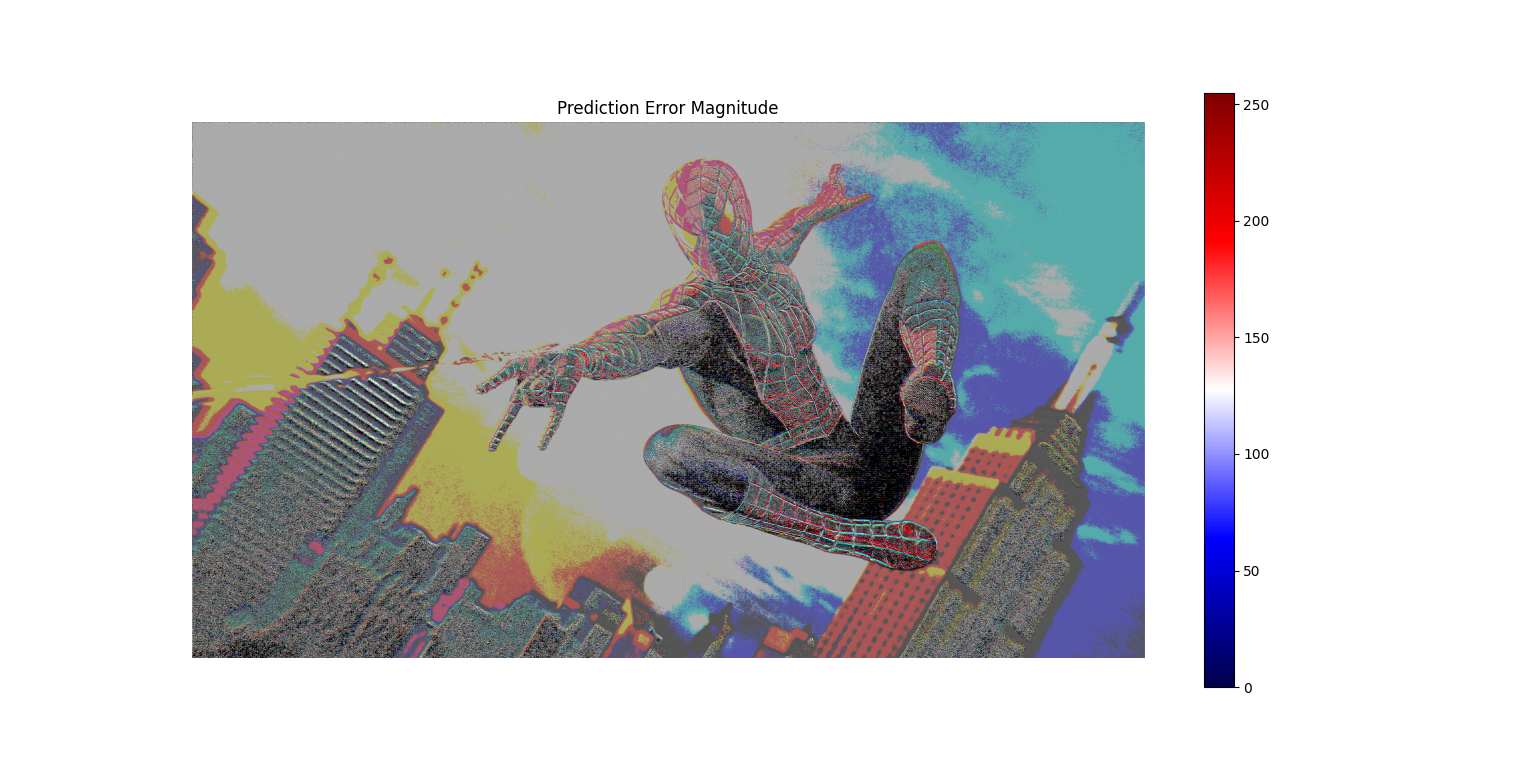
\includegraphics[width = .9\textwidth]{hw-1/report/imgs/advanced-coding.png}
    \caption{Rappresentazione del modulo dell'errore di predizione nella codifica avanzata.}
    \label{fig:advanced-coding}
\end{figure}

\FloatBarrier\noindent Si osserva che per quanto l'immagine \ref{fig:advanced-coding} sia simile alla figura \ref{fig:simple-coding}, è presente una differenza: è sufficente mostrare un'immagine che contenga la differenza in modulo tra le varaibili \texttt{adv\_coding\_error} e \texttt{simple\_coding\_error}. Dal risultato, mostrato nella figura \ref{fig:error-difference}, si può notare che non è di colore uniforme ma presenta diverse sfumature di blu, suggerendo quindi una bassa differenza tra le due che quindi le rende non identiche.

\begin{figure}[h]
    \centering
    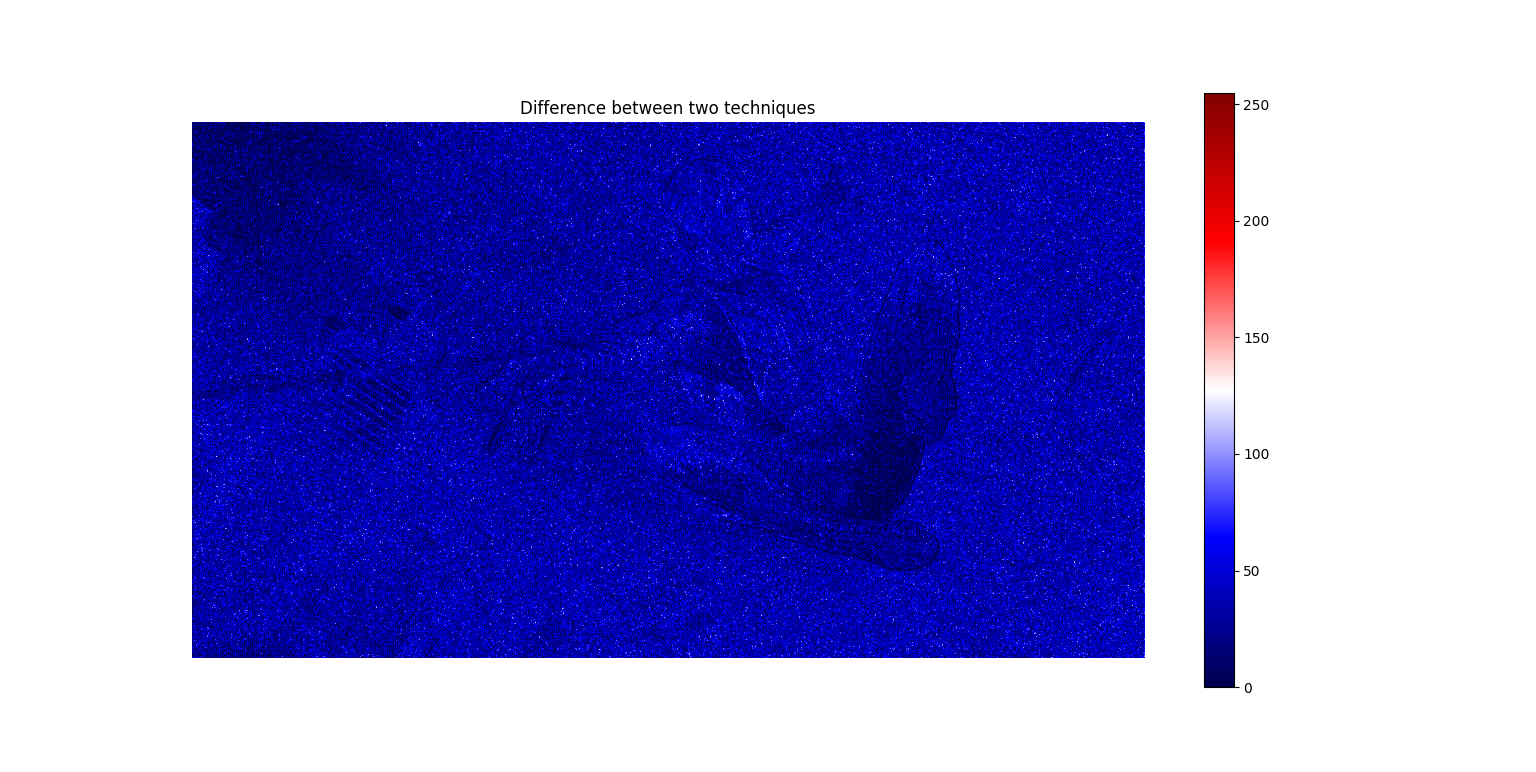
\includegraphics[width = .9\textwidth]{hw-1/report/imgs/error-difference.png}
    \caption{Rappresentazione della differenza tra l'errore della codifica semplice e della codifica avazata.}
    \label{fig:error-difference}
\end{figure}



\subsubsection{Analisi}\todo{valuta se farla subsection}





\vspace{30px}\section{Conclusioni}




\begin{comment}

    (1) Entropia b&w:       7.530 bpp
    (2) Bitrate .zip:       1.340 bpp
    (3) discussion
    (4) simple-coding-img
    (5) Bitrate EG:         10.0135 bpp
    (6) advanced-coding-img
    (7) Bitrate EG:         9.7443 bpp

\end{comment}

\end{document}
